\renewcommand{\theequation}{\theenumi}
\begin{enumerate}[label=\arabic*.,ref=\thesubsection.\theenumi]
\item The equation of a circle is 
\begin{align}
\label{eq:circ_norm}
\norm{\vec{x}-\vec{c}} = r
\end{align}
%
where $\vec{c}$ is the centre and $r$ is the radius.
\item By expanding \eqref{eq:circ_norm}, the equation of a circle can also be expressed as
%
\numberwithin{equation}{enumi}
\begin{align}
\norm{\vec{x}-\vec{c}}^2 = r^2&
\\
\implies \vec{x}^T\vec{x}-2\vec{c}^T\vec{x} + \vec{c}^T\vec{c}-r^2 = 0
\label{eq:circ_quad}
\end{align}
\item The direction vector of {\em normal to the circle}  in \eqref{eq:circ_quad} at point $\vec{p}$ is
\begin{align}
\label{eq:circ_normal}
\vec{n} = k\brak{\vec{p}-\vec{c}},
\end{align}
%
where $k$ is a constant.
\item Find the equation of a circle that passes through the points $\vec{A},\vec{B},\vec{C}$.
\\
\solution From \eqref{eq:circ_quad},
\begin{align}
%\label{eq:circ_quad}
\norm{\vec{A}-\vec{c}}^2 = \norm{\vec{B}-\vec{c}}^2 = \norm{\vec{C}-\vec{c}}^2 &= r^2
\\
\implies \norm{\vec{A}-\vec{c}}^2 - \norm{\vec{B}-\vec{c}}^2 &=0
\end{align}
which can be simplified to obtain
\begin{align}
\brak{\vec{A}-\vec{B}}^T\vec{c}=\frac{\norm{\vec{A}}^2 - \norm{\vec{B}}^2}{2}& \quad \text{and}
\\
\brak{\vec{A}-\vec{C}}^T\vec{c}=\frac{\norm{\vec{A}}^2 - \norm{\vec{C}}^2}{2}& 
\end{align}
%
Solving the two yields $\vec{c}$, which can then be used to obtain $r$.
\item Let $\vec{A},\vec{B}$ and $\vec{C}$ be three points on the circle and 
$D$ be a point on $BC$ such that
$OD \perp BC$ as in Fig. \ref{fig:ccircle}.  Show that 
\begin{align}
\vec{D}=\frac{\vec{B}+\vec{C}}{2}
\end{align}
%
\begin{figure}[!ht]
	\begin{center}
		
		%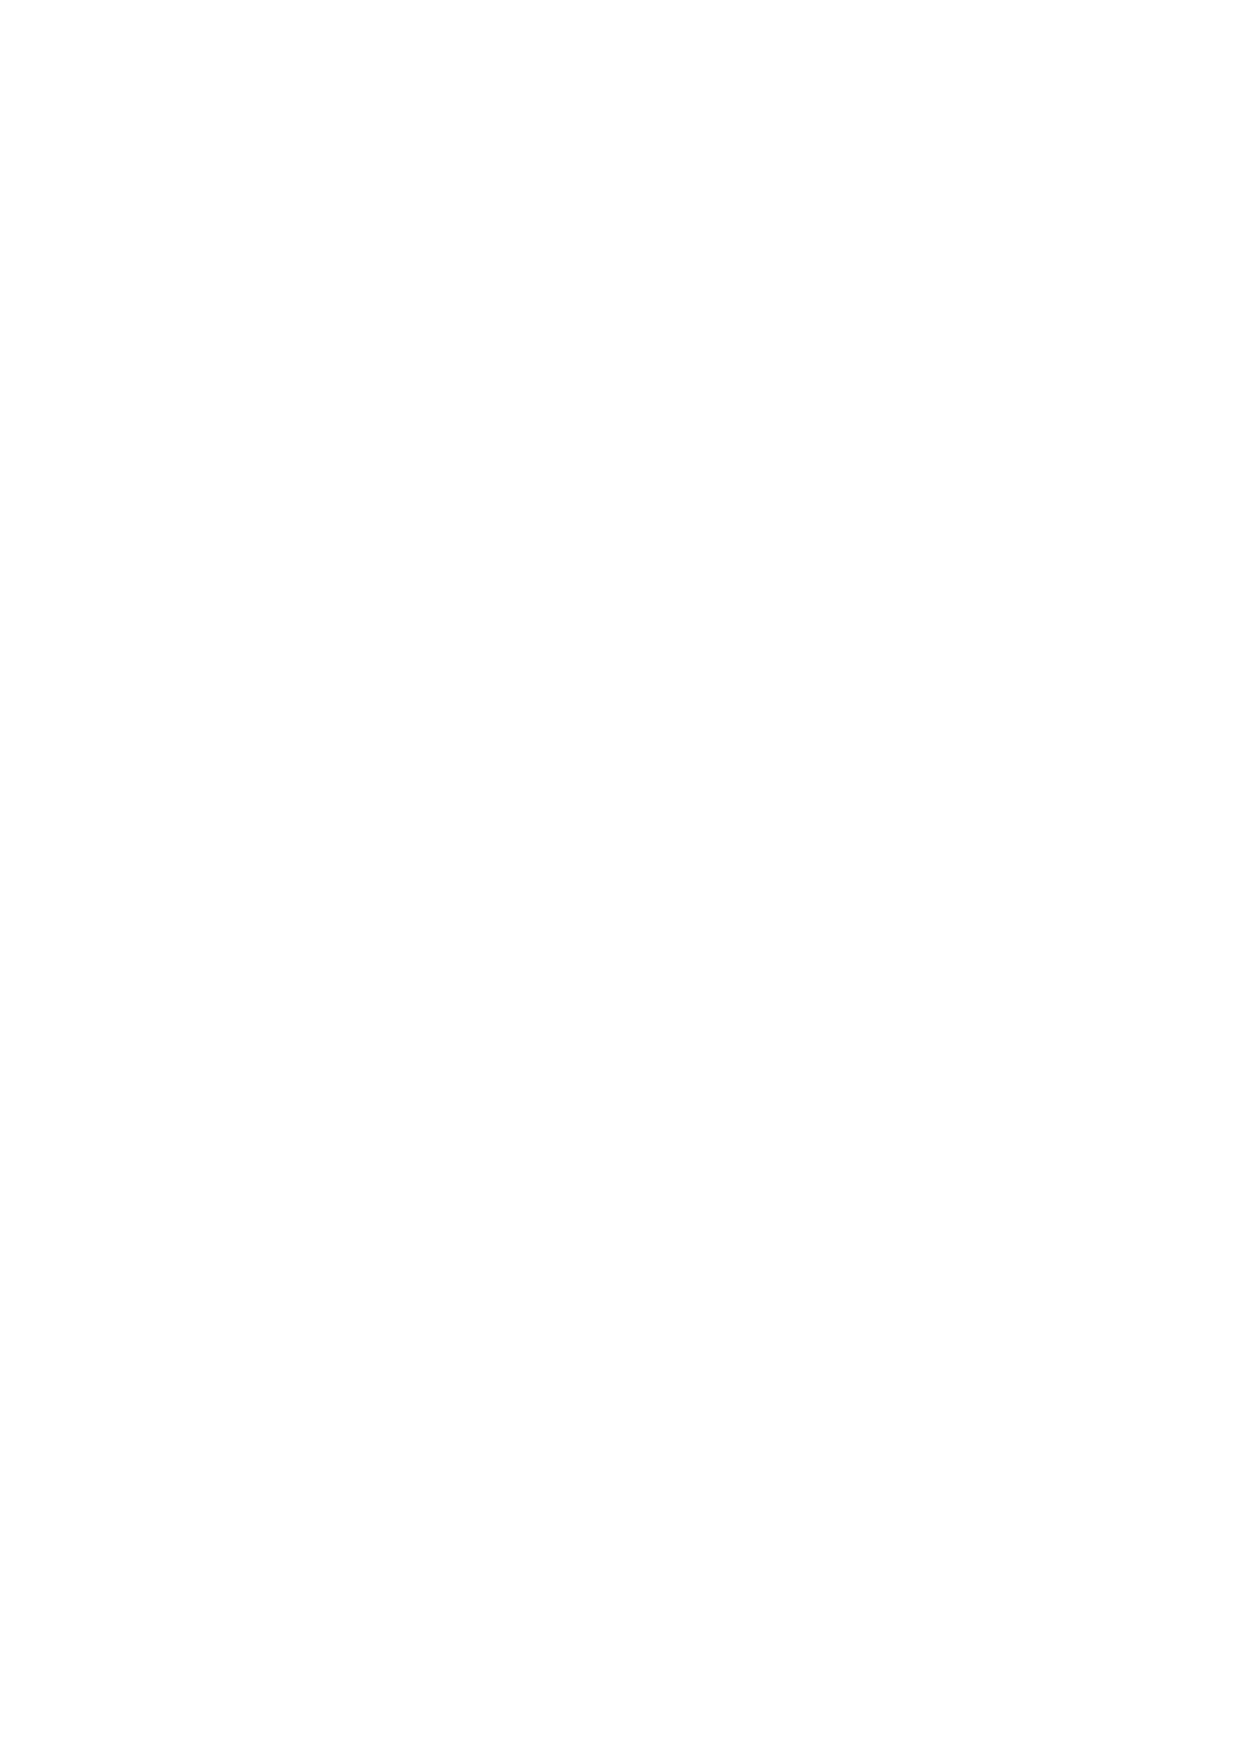
\includegraphics[width=\columnwidth]{./figs/ch3_angle_bisector}
		%\vspace*{-10cm}
		\resizebox{\columnwidth}{!}{\begin{tikzpicture}
[scale=2,>=stealth,point/.style={draw,circle,fill = black,inner sep=0.5pt},]

%\node (D) at (0, 0)[point,label=below :$D$] {};
\node (B) at (-2, -2)[point,label=below left :$B$]{};
\node (A) at (1, 3)[point,label=above:$A$]{};
\node (C) at (4, -1)[point,label=below right:$C$]{};
%\coordinate [point, label={above : $O$ }] (I) at  (1.147, 1.143);
\node (O) at (0.7962963,-0.27777778)[point,label=above:$O$]{};
\node (D) at ( 1,-1.5)[point,label=below:$D$]{};
%\node (x1) at (0.601,-1.357)[point,label=left:$x_1$]{};
%\node (x2) at (2.15,-1.1)[point,label=right:$x_2$]{};
%\node (temp) at ($(O)!0.5!(D)$)[label=right:$r$]{};
%\node (D) at (2.424,1.1)[point,label=above right:$D$]{};
%\node (E) at (1.1, 1.9)[point,label=above right:$E$]{};
%\node (F) at (-1.1, 1.9)[point,label=above left:$F$]{};
\def\rad{3.284101453883}
\draw (O) circle (\rad);

\draw (D)--(O);
\draw (A)--(B);
\draw (B)--(C);
\draw (A)--(C);
%\draw (C)--(D);
%\draw [thick,dashed] (x1) -- (x2);
%\draw [thick,dashed] (O) -- (E);
%\draw [thick,dashed] (O) -- (F);
%\draw (B)--(O);
%\draw (C)--(O);

%\tkzMarkRightAngle[size=.2](A,D,C)
%\tkzMarkRightAngle[size=.15](B,F,O);
%\tkzMarkRightAngle[size=.15](C,E,O);
%\tkzMarkAngle[size=.4](D,B,O);
%\tkzMarkAngle[size=.35](O,B,F);
%\tkzMarkAngle[size=.54](E,C,O);
%\tkzMarkAngle[size=.5](E,C,O);
%\tkzMarkAngle[size=.6](O,C,D);
%\tkzMarkAngle[size=.65](O,C,D);

\end{tikzpicture}}
	\end{center}
	\caption{Circumcircle.}
	\label{fig:ccircle}	
\end{figure}


\solution From \eqref{eq:circ_norm}
\begin{align}
\norm{\vec{B}-\vec{O}}^2=\norm{\vec{C}-\vec{O}}^2=r^2
\\
 \implies \brak{\vec{B}-\vec{O}}^T\brak{\vec{B}-\vec{O}} = 
\brak{\vec{C}-\vec{O}}^T\brak{\vec{C}-\vec{O}} 
\\
 \implies \brak{\vec{B}-\vec{C}}^T\brak{\frac{\vec{B}+\vec{C}}{2} - 
\vec{O}}  = 0
\label{eq:circle_mid}
\end{align}
after simplification. Since $OD \perp BC$,
\begin{align}
\brak{\vec{B}-\vec{C}}^T\brak{\vec{D}-\vec{O}} = 0 
\label{eq:circle_D}
\end{align}
Since $D$ and $\frac{\vec{B}+\vec{C}}{2}$ lie on $BC$, using 
\eqref{eq:line_ab},
\begin{align}
\label{eq:circle_mid_D1}
\frac{\vec{B}+\vec{C}}{2}
&= \vec{B}+ \lambda_1\brak{\vec{B}-\vec{C}}
\\
\vec{D}
&= \vec{B}+ \lambda_2\brak{\vec{B}-\vec{C}}
\label{eq:circle_mid_D2}
\end{align}
Multiplying \eqref{eq:circle_mid_D1} and \eqref{eq:circle_mid_D2} with 
$\brak{\vec{B}-\vec{C}}^T$ and subtracting, $\lambda_1=\lambda_2$
%
\begin{align}
\implies \vec{D} = \frac{\vec{B}+\vec{C}}{2}
\label{eq:circle_bisect}
\end{align}
%
\item Let  $\vec{D}$ be the mid point of $BC$.  Show that $OD \perp BC$.
%
\item The circle with centre $\vec{O}$ and radius $r$ in Fig.\ref{fig:ang_bisect}	
 is inside 
$\triangle ABC$ and touches $AB, BC$ 
and $CA$ at $\vec{F}, \vec{D}$ and $\vec{E}$ respectively. $AB, BC$ and 
$CA$ are known as {\em tangents} to the circle.
\begin{figure}[!ht]
	\begin{center}
		
		%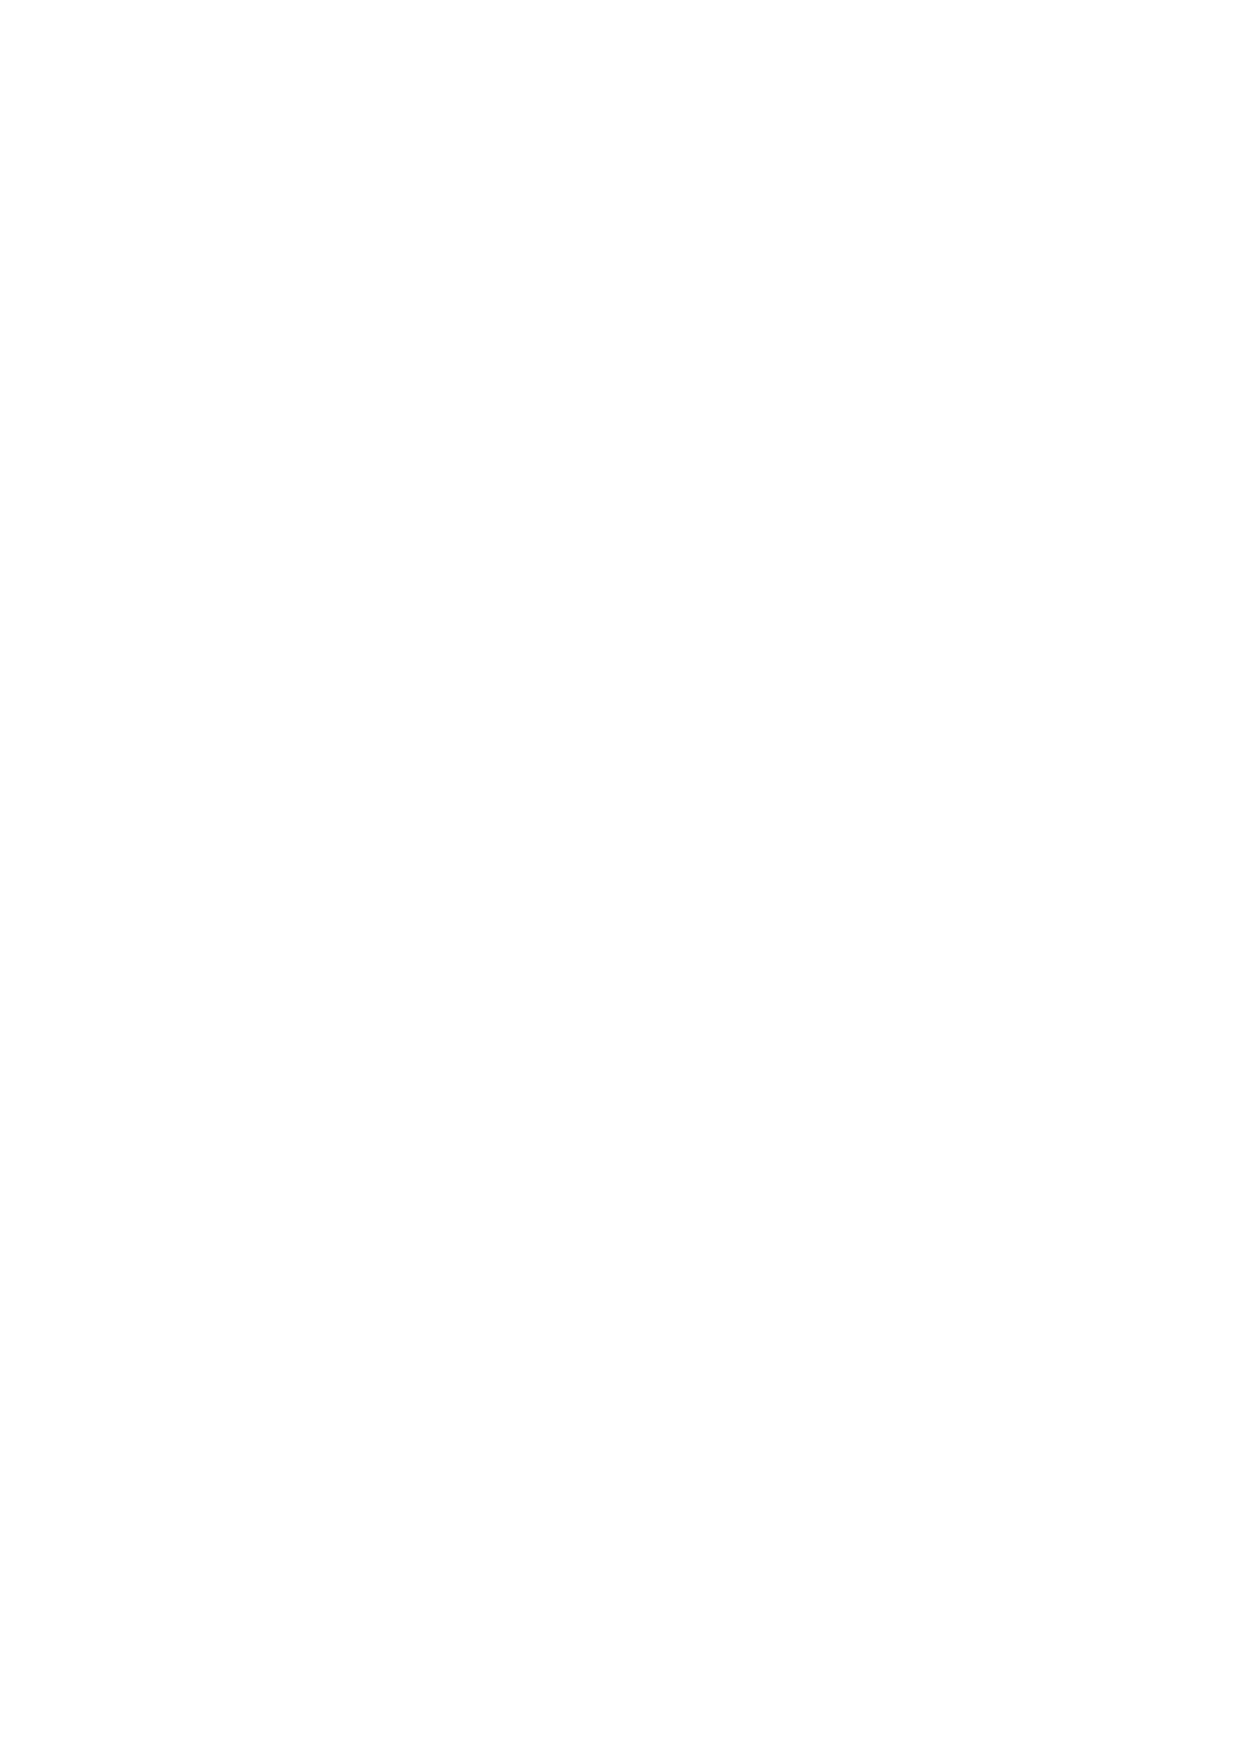
\includegraphics[width=\columnwidth]{./figs/ch3_angle_bisector}
		%\vspace*{-10cm}
		\resizebox{\columnwidth}{!}{\begin{tikzpicture}
[scale=2,>=stealth,point/.style={draw,circle,fill = black,inner sep=0.5pt},]

%\node (D) at (0, 0)[point,label=below :$D$] {};
\node (B) at (-2, -2)[point,label=below left :$B$]{};
\node (A) at (1, 3)[point,label=above:$A$]{};
\node (C) at (4, -1)[point,label=below right:$C$]{};
%\coordinate [point, label={above : $O$ }] (I) at  (1.147, 1.143);
\node (O) at (1.147, 0.143)[point,label=above:$I$]{};
\node (D) at (1.41,-1.43)[point,label=below:$U$]{};
\node (x1) at (0.601,-1.357)[point,label=left:$x_1$]{};
\node (x2) at (2.15,-1.1)[point,label=right:$x_2$]{};
\node (temp) at ($(O)!0.5!(D)$)[label=right:$r$]{};
%\node (D) at (2.424,1.1)[point,label=above right:$D$]{};
%\node (E) at (1.1, 1.9)[point,label=above right:$E$]{};
%\node (F) at (-1.1, 1.9)[point,label=above left:$F$]{};
\def\rad{1.596}
\draw (O) circle (\rad);

\draw (D)--(O);
\draw (A)--(B);
\draw (B)--(C);
\draw (A)--(C);
%\draw (C)--(D);
\draw [thick,dashed] (x1) -- (x2);
%\draw [thick,dashed] (O) -- (E);
%\draw [thick,dashed] (O) -- (F);
%\draw (B)--(O);
%\draw (C)--(O);

%\tkzMarkRightAngle[size=.2](A,D,C)
%\tkzMarkRightAngle[size=.15](B,F,O);
%\tkzMarkRightAngle[size=.15](C,E,O);
%\tkzMarkAngle[size=.4](D,B,O);
%\tkzMarkAngle[size=.35](O,B,F);
%\tkzMarkAngle[size=.54](E,C,O);
%\tkzMarkAngle[size=.5](E,C,O);
%\tkzMarkAngle[size=.6](O,C,D);
%\tkzMarkAngle[size=.65](O,C,D);

\end{tikzpicture}
}
	\end{center}
	\caption{Tangent and incircle.}
	\label{fig:ang_bisect}	
\end{figure}


\item Show that $OD \perp BC$.
%\begin{figure}[!h]
%\centering
%\resizebox {\columnwidth} {!} {
%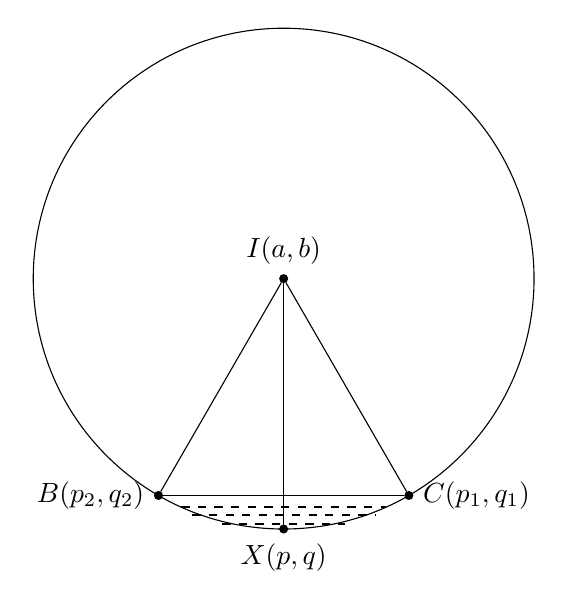
\begin{tikzpicture}
[
scale =2,
>=stealth,
point/.style = {draw, circle, fill = black, inner sep = 1pt},
]

\def\rad{1.59}
\coordinate [point, label={above : $I{(a,b)}$ }] (I) at (0, 0);
\draw (I) circle (\rad);

\node (C) at (300:{\rad})[point,label = right:$C{(p_1,q_1)}$] {};

\node (X) at (270:{\rad}) [point,label = below:$X{(p,q)}$] {};

\node (B) at (240:{\rad}) [point,label = left:$B{(p_2,q_2)}$] {};

\draw (C) -- (I);
\draw (B) -- (I);
\draw (B) -- (C);
\draw (I) -- (X);

\draw[black,thick,dashed](-0.65,-1.45) -- (0.65,-1.45);
\draw[black,thick,dashed](-0.58,-1.5) -- (0.58,-1.5);
\draw[black,thick,dashed](-0.39,-1.56) -- (0.39,-1.56);
\end{tikzpicture}

%}
%\caption{Notion of the derivative.}
%\label{fig:derivative}
%\end{figure}
\\
\solution Let $\vec{x}_1,\vec{x}_2$ be two points on the circle such that 
$x_1x_2 \parallel BC$. Then
%
\begin{align}
\norm{\vec{x}_1-\vec{O}}^2- 
\norm{\vec{x}_2-\vec{O}}^2 &= 0 
\\
\implies 
\brak{\vec{x}_1-\vec{x}_2}^T\brak{\frac{\vec{x}_1+\vec{x}_2}{2}-\vec{O}} &= 
0 
\\
\implies 
\brak{\vec{B}-\vec{C}}^T\brak{\frac{\vec{x}_1+\vec{x}_2}{2}-\vec{O}} &= 
0 
%\label{eq:circle_bisect}
\end{align}
%
For $\vec{x}_1=\vec{x}_2=\vec{D}$, $x_1x_2$ merges into $BC$ and the above 
equation becomes 
%
\begin{align}
\brak{\vec{B}-\vec{C}}^T\brak{\vec{D}-\vec{O}} = 
0 
\implies OD \perp BC
%\label{eq:circle_bisect}
\end{align}
%
\item Give an alternative proof for the above.
\\
\solution Let 
\begin{align}
\vec{B} & = \mbf{0}
\\
\vec{D} &= \lambda \vec{m}
\end{align}
Then
\begin{align}
\norm{\vec{D} - \vec{O}}^2 = r^2 &
\\
\implies \lambda^2\norm{\vec{m}}^2 - 2\lambda\vec{m}^T\vec{O} + \norm{\vec{O}}^2 &= r^2 
\end{align}
Since the above equation has a single root,
\begin{align}
\lambda = \frac{\vec{m}^T\vec{O}}{\norm{\vec{m}}^2}
\label{eq:incircle_lam}
\end{align}
%
Thus, 
\begin{align}
\brak{\vec{D} - \vec{B}}^T\brak{\vec{D} - \vec{O}}
&= \brak{\lambda\vec{m}}^T
\brak{\lambda\vec{m}-\vec{O}}
\\
&=\lambda^2\norm{\vec{m}}^2-\lambda\vec{m}^T\vec{O}
\\
&= \mbf{O} \text{ (from \ref{eq:incircle_lam})}.
\\
\implies & OD \perp BC
\end{align}
\item Find the equation of the tangent at $\vec{D}$.
\\
\solution The equation of the tangent is given by 
\begin{align}
\brak{\vec{O}-\vec{D}}^T\brak{\vec{x}-\vec{D}}=0
%\label{eq:circle_bisect}
\end{align}
%
\item Show that the angle in a semi-circle is a right angle.
\begin{figure}[!h]
\centering
\resizebox {\columnwidth} {!} {
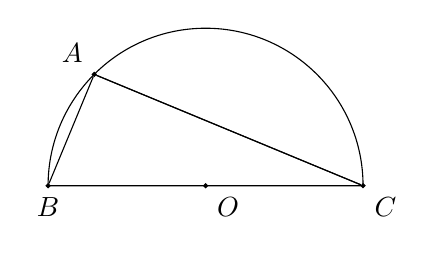
\begin{tikzpicture}
  [
    scale=2,
    >=stealth,
    point/.style = {draw, circle,  fill = black, inner sep = 0.5pt},
    dot/.style   = {draw, circle,  fill = black, inner sep = .2pt},
  ]

 \coordinate [point, label={below :	$B$ }] (B) at (-1, 0);
 \coordinate [point, label={below right:	$O$ }] (O) at (0, 0);
 \coordinate [point, label={below right:	$C$ }] (C) at (1, 0); 
 \coordinate [point, label={above left:	$A$ }] (A) at (-0.707,0.707);  
\draw (A) -- (C) arc(0:180:1) --cycle;
  \draw 
  (A) -- (B)
  (A) -- (C);
  \tkzMarkRightAngle[fill=blue!20,size=.2](B,A,C)    
%  \def\rad{1}

%  \draw (O) circle (\rad);  
%    \node (A) at +(45:{\rad}) [point,label = above right:$A$ $\brak{x,y}$] {};  
%  \path
%     (O)    edge  node[sloped, anchor=center, below, text width=0.5cm] { $r$}     (A) ; 
    
% \coordinate [point, label={below left:$B$}] (B) at (0, 0);
%    \node (A) at +(60:{2*sqrt(3)}) [label = above:$A$] {};
%  \coordinate [ label={below right:$C$ }] (C) at ($ (3,0) + sqrt(3)*(1,0) $);
%    \node (P) at +(30:{2*sqrt(3)}) [label = above:$P$] {};  
%  \path[->]
%     (B)    edge  node[sloped, anchor=center, below, text width=2.0cm] { $y = m_1x+c_1$}     (A) 
%	 (B)    edge  node[sloped, anchor=east, below, text width=2.0cm] { $y=m_2x+c_2$}     (C)
%	 (B)    edge  node[sloped, anchor=east, below, text width=2.0cm] { Bisector}     (P);
%  
%%  
%%  \coordinate [point, label={below left:$B$ $\brak{0,0}$}] (B) at (0, 0);
%%    \node (A) at +(60:{2*sqrt(3)}) [point, label = above:$A$ $\brak{a,b}$] {};
%%  \coordinate [point, label={below right:$C$ $\brak{c,0}$}] (C) at ($ (3,0) + sqrt(3)*(1,0) $);
%%  \node (D) at ({sqrt(3)},0) [point, label = below:$D$ $\brak{a,0}$] {};
%%    \node (E) at +(45:{(3+sqrt(3))/sqrt(2)}) [point, label = above right:$E$] {};
%%    \node (O) at +(45:{sqrt(6)}) [point, label = right:$O$] {};    
%%    \node (F) at +(60:{(3+sqrt(3))/2}) [point, label = left:$F$] {};        
%  \draw  (A) -- (B) -- (C);% -- (A);
%%  \node (D) at ($(B)!0.5!(C)$) [point, label = {below:$D$}]{};
%%  \draw (A) -- (D);  
%%  \draw (B) -- (E);    
%%  \draw[dashed] (C) -- (F);      
%\tkzMarkAngle[draw = black, fill = white, opacity=1](P,B,A)
%\tkzLabelAngle[pos = 0.8](P,B,A){$\theta$}
%\tkzMarkAngle[draw = black, fill = white, opacity=1,size=1.1](C,B,P)
%\tkzLabelAngle[pos = 0.9](C,B,P){$\theta$}

%\tkzMarkAngle[size=1.4,draw = black, fill = white, opacity=1](C,B,P)
%\tkzLabelAngle[pos=1.15,font=\scriptsize](C,B,P){$\theta$}

%  \tkzMarkAngle[fill=white,opacity=1,size=0.2,label={$\theta$},pos=0.2](P,B,A)  
%  \tkzMarkAngle[fill=blue!20,size=.4,label={$\theta$}](P,B,A)
%  \tkzMarkAngle[fill=blue!20,size=.2,label={$\theta$](C,B,P)
%  \tkzMarkRightAngle[fill=blue!20,size=.2](B,E,A)  
%  \path
%     (B)    edge  node[sloped, anchor=center, below, text width=2.0cm] { $k_1:1$}     (E)  
%	 (C)    edge  node[sloped, anchor=east, below, text width=2.0cm] { $1:k_2$}     (F);

\end{tikzpicture}


}
\caption{Angle in a semi-circle.}
\label{fig:ch2_line}
\end{figure}
\\
\solution Let 
\begin{align}
\vec{O} = 0
\end{align}
From the given information,
\begin{align}
\label{eq:semi_circ_pt}
\norm{\vec{A}}^2 = \norm{\vec{B}}^2 = \norm{\vec{C}}^2 = r^2
\\
\norm{\vec{B}-\vec{C}}^2 =  \brak{2r}^2
\\
\vec{B} + \vec{C} = 0
\label{eq:semcirc_mid}
\end{align}
%
where $r$ is the radius of the circle. Thus,
\begin{multline}
\norm{\vec{A}-\vec{B}}^2 + \norm{\vec{A}-\vec{C}}^2 = 
2\norm{\vec{A}}^2 + \norm{\vec{B}}^2 + \norm{\vec{C}}^2
\\
-2\vec{A}^T\brak{\vec{B}+\vec{C}}
%\\
%\norm{\vec{B}-\vec{C}}^2 =  \brak{2r}^2
%\\
%\vec{B} + \vec{C} = 0
\end{multline}
From \eqref{eq:semcirc_mid} and \eqref{eq:semi_circ_pt},
\begin{multline}
\norm{\vec{A}-\vec{B}}^2 + \norm{\vec{A}-\vec{C}}^2 = 4r^2 = \norm{\vec{B}-\vec{C}}^2 
%\\
%\norm{\vec{B}-\vec{C}}^2 =  \brak{2r}^2
%\\
%\vec{B} + \vec{C} = 0
\end{multline}
Thus, using Baudhayana's theorem, $\triangle ABC$ is right angled.
\item 	Show that $PA.PB = PC^2$, where $PC$ is the tangent to the circle in Fig. \ref{fig:tangent_secant}.

	\begin{figure}[!hb]
		\begin{center}
			
			%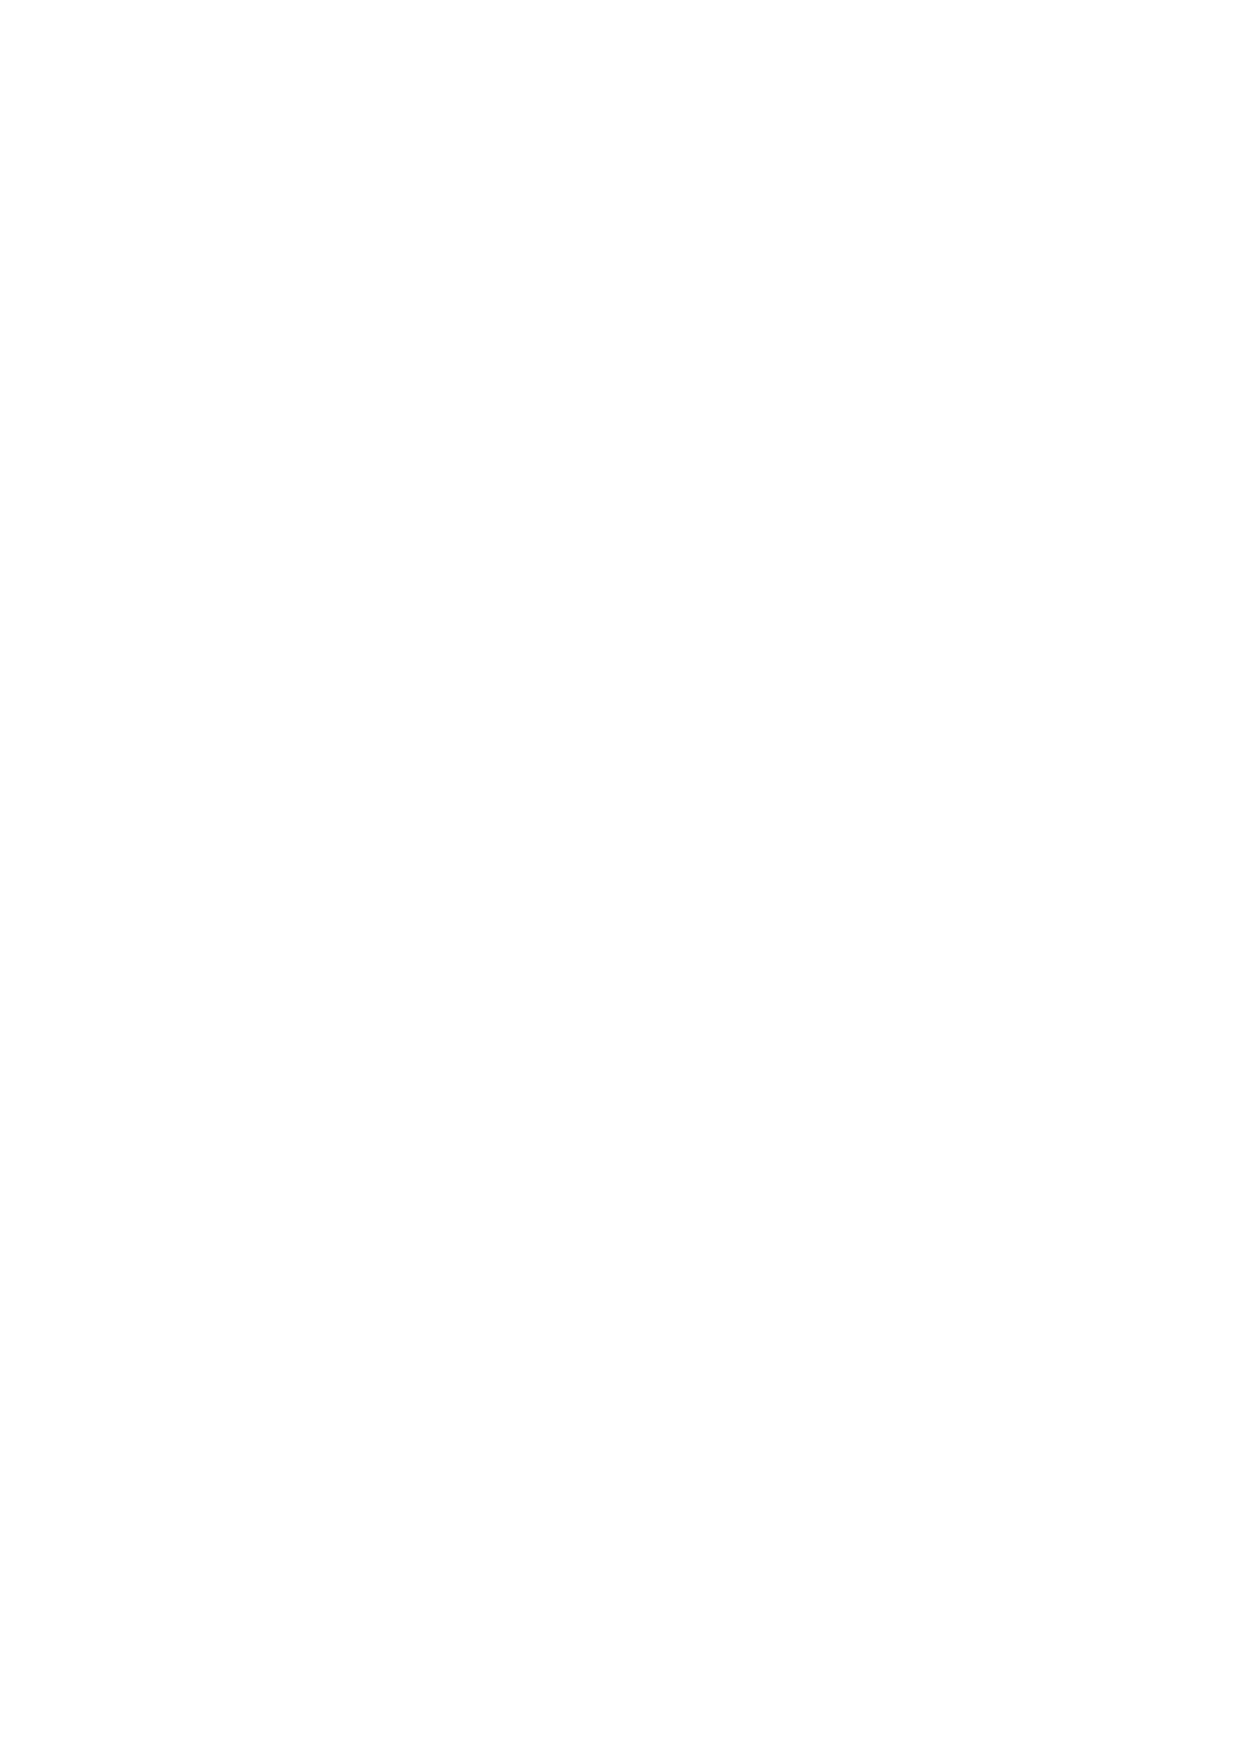
\includegraphics[width=\columnwidth]{./figs/ch4_tangent_prod}
			%\vspace*{-10cm}
			\resizebox{\columnwidth}{!}{\begin{tikzpicture}
[scale =2,>=stealth,point/.style = {draw, circle, fill = black, inner sep = 1pt},]

\def\rad{2}
\coordinate [point, label={above: $O$ }] (O) at (0, 2);
\draw (O) circle (\rad);
\node (P) at (-4,0)[point,label=below :$P$] {};
\node (C) at (0,0)[point,label=below :$C$] {};
\node (A) at (-1.92,1.45)[point,label=above left :$A$] {};
\node (B) at (1.2,3.6)[point,label=above right :$B$] {};
\draw (O)--(P);
\draw (P)--(C);
\draw (P)--(B);
%\draw (A)--(O);
%\draw (B)--(C);

\draw [thick,dashed](A)--(O);
\draw [thick,dashed](C)--(O);
\draw [thick,dashed](B)--(O);
%\tkzMarkRightAngle[size=.2](P,C,O);
%\tkzMarkAngle[size=.3](A,B,C);
%\tkzMarkAngle[size=.4](O,C,A);
%\tkzMarkAngle[size=.5](B,C,O);
%\tkzMarkAngle[size=.3](P,A,C);
%\tkzMarkAngle[size=.2](C,A,O);
%\tkzMarkAngle[size=.2](A,O,C);
%
\node [above] at (0.35,2.5){$r$};
\node [above] at (-0.9,1.7){$r$};
\node [above] at (0.1,1.0){$r$};
%\draw (-1.9,1) node{$\theta$};

%\draw (0.95,3.3) node{$\alpha$};
%\draw (-0.2,1.7) node{$2\alpha$};
%\draw (-0.2,0.5) node{$90-\alpha$};
%\draw (-1.4,1.4) node{$90-\alpha$};
%\draw (.1,.6) node{$\phi$};

\end{tikzpicture}}
		\end{center}
		\caption{$PA.PB = PC^2$.}
		\label{fig:tangent_secant}	
	\end{figure}
\solution Let $\vec{P} = \mbf{0}$.  Then, we have the following equations
\begin{align}
\label{eq:tan_sec_AB}
PA.PB &= \lambda \norm{\vec{A}}^2 \quad \because (\vec{B} = \lambda \vec{A})
\\
\norm{\vec{A}-\vec{O}}^2 &= \norm{\vec{B}-\vec{O}}^2 = \norm{\vec{C}-\vec{O}}^2 = r^2
\\
\norm{\vec{O}}^2-\norm{\vec{C}}^2 &=  r^2 \quad \triangle PCO\text{ is 
right angled}
\label{eq:tan_sec_boudh}
\end{align}
$\because$
\begin{align}
%\label{eq:tan_sec_AB}
%PA.PB &= \lambda \norm{\vec{A}}^2 \quad \because (\vec{B} = \lambda 
%\vec{A})
%\\
\norm{\vec{B}-\vec{O}}^2-\norm{\vec{A}-\vec{O}}^2   &=0,
\\
\brak{\lambda^2-1}\norm{\vec{A}}^2 - 2 \brak{\lambda-1}\vec{A}^T\vec{O} &= 
0
\\
\implies PA.PB = \lambda\norm{\vec{A}}^2 =  2 
\vec{A}^T\vec{O}-\norm{\vec{A}}^2 &
%\norm{\vec{C}-\vec{O}}^2 = r^2
%\\
%\norm{\vec{O}}^2-\norm{\vec{C}}^2 &=  r^2 \quad \triangle PCO\text{ is 
%right angled}
%\label{eq:tan_sec_boudh}
\label{eq:tan_sec_first}
\end{align}
after substituting from \eqref{eq:tan_sec_AB} and simplifying. From 
\eqref{eq:tan_sec_boudh},
\begin{align}
\norm{\vec{A}-\vec{O}}^2 = \norm{\vec{O}}^2-\norm{\vec{C}}^2  &= r^2
\\
\implies 2 \vec{A}^T\vec{O}-\norm{\vec{A}}^2   = \norm{\vec{C}}^2 = PC^2&
\label{eq:tan_sec_second}
\end{align}
From \eqref{eq:tan_sec_first} and \eqref{eq:tan_sec_second},
\begin{align}
PA.PB = PC^2
\end{align}

\item In Fig. \ref{fig:chords} show that $PA.PB = PC.PD$.
\begin{figure}[!ht]
	\begin{center}
		
		%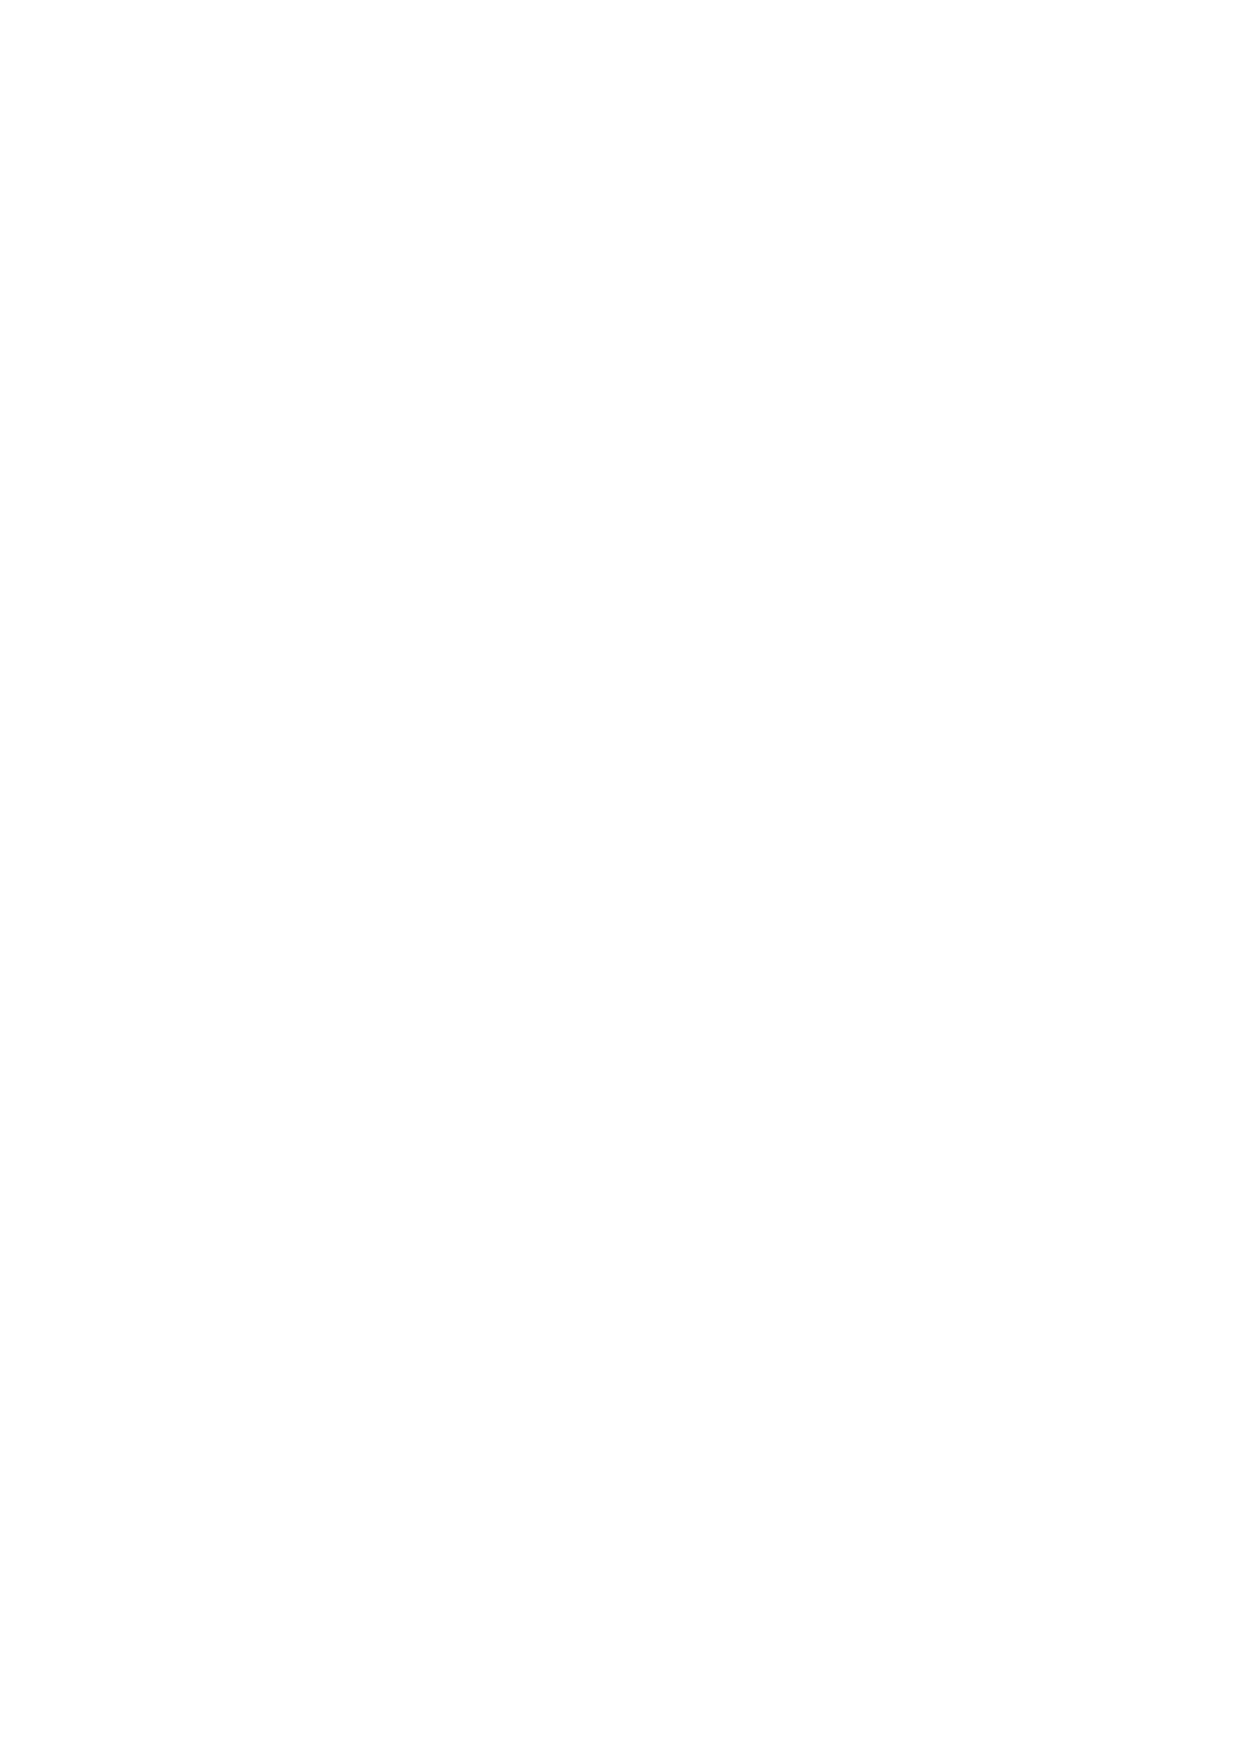
\includegraphics[width=\columnwidth]{./figs/ch3_angle_bisector}
		%\vspace*{-10cm}
		\resizebox{\columnwidth}{!}{\begin{tikzpicture}
[scale=2,>=stealth,point/.style={draw,circle,fill = black,inner sep=0.5pt},]
%\node (D) at (0, 0)[point,label=below :$D$] {};
\node (B) at (-2, -2)[point,label=below left :$C$]{};
\node (A) at (1, 3)[point,label=above:$A$]{};
\node (C) at (4, -1)[point,label=below right:$B$]{};
%\coordinate [point, label={above : $O$ }] (I) at  (1.147, 1.143);
\node (O) at (0.7962963,-0.27777778)[point,label=above:$O$]{};
\node (D) at (  3.64041158, 1.36427295)[point,label=below:$D$]{};
\node (P) at ( 2.66371481, 0.78171359)[point,label=right:$P$]{};
%\node (x1) at (0.601,-1.357)[point,label=left:$x_1$]{};
%\node (x2) at (2.15,-1.1)[point,label=right:$x_2$]{};
%\node (temp) at ($(O)!0.5!(D)$)[label=right:$r$]{};
%\node (D) at (2.424,1.1)[point,label=above right:$D$]{};
%\node (E) at (1.1, 1.9)[point,label=above right:$E$]{};
%\node (F) at (-1.1, 1.9)[point,label=above left:$F$]{};
\def\rad{3.284101453883}
\draw (O) circle (\rad);

%\draw (D)--(O);
%\draw (A)--(B);
\draw (B)--(D);
\draw (A)--(C);
%\draw (C)--(D);
%\draw [thick,dashed] (x1) -- (x2);
%\draw [thick,dashed] (O) -- (E);
%\draw [thick,dashed] (O) -- (F);
%\draw (B)--(O);
%\draw (C)--(O);

%\tkzMarkRightAngle[size=.2](A,D,C)
%\tkzMarkRightAngle[size=.15](B,F,O);
%\tkzMarkRightAngle[size=.15](C,E,O);
%\tkzMarkAngle[size=.4](D,B,O);
%\tkzMarkAngle[size=.35](O,B,F);
%\tkzMarkAngle[size=.54](E,C,O);
%\tkzMarkAngle[size=.5](E,C,O);
%\tkzMarkAngle[size=.6](O,C,D);
%\tkzMarkAngle[size=.65](O,C,D);

\end{tikzpicture}}
	\end{center}
	\caption{Chords of a circle}
	\label{fig:chords}	
\end{figure}
\\
\solution Let $\vec{P} = \mbf{0}$.  We then have the following equations
\begin{align}
\begin{split}
\vec{B} &= k_1 \vec{A}, k_1 = \frac{PB}{PA}
\\
\vec{D} &= k_2 \vec{C}, k_2 = \frac{PD}{PC}
\end{split}
\label{eq:chords_ratio}
\\
\begin{split}
\norm{\vec{A}-\vec{O}}^2 &= \norm{\vec{B}-\vec{O}}^2 
\\
= \norm{\vec{C}-\vec{O}}^2 &= \norm{\vec{D}-\vec{O}}^2 = r^2
\end{split}
\label{eq:chords_points}
\end{align}
%
where $r$ is the radius of the circle and $\vec{O}$ is the centre. From \eqref{eq:chords_points},
\begin{align}
&\norm{\vec{A}-\vec{O}}^2 = \norm{\vec{B}-\vec{O}}^2
\\
\implies &\norm{\vec{A}-\vec{O}}^2 = \norm{k\vec{A}-\vec{O}}^2 \quad(\text{from \eqref{eq:chords_ratio}})
\end{align}
%
which can be simplified to obtain
\begin{align}
k_1\norm{\vec{A}}^2 = 2\vec{A}^T\vec{O}-\norm{\vec{A}}^2
\label{eq:chords_Anorm}
\end{align}
Similarly,
\begin{align}
k_2\norm{\vec{C}}^2 = 2\vec{C}^T\vec{O}-\norm{\vec{C}}^2
\label{eq:chords_Cnorm}
\end{align}
%
From \eqref{eq:chords_points}, we also obtain
\begin{align}
\norm{\vec{A}-\vec{O}}^2 
= \norm{\vec{C}-\vec{O}}^2 
\\
\implies 2\vec{A}^T\vec{O}-\norm{\vec{A}}^2 = 2\vec{C}^T\vec{O}-\norm{\vec{C}}^2
\label{eq:chords_ACnorm}
\end{align}
%
after simplification. Using this result in \eqref{eq:chords_Anorm} and \eqref{eq:chords_Cnorm},
\begin{align}
k_1\norm{\vec{A}}^2 = k_2\norm{\vec{C}}^2
\\
\implies \norm{\vec{A}}\, \norm{\vec{B}}=\norm{\vec{C}}\,\norm{\vec{D}}
\end{align}
which completes the proof.

\item (Pole and Polar:) The polar of a point $\vec{x}$ with respect to the curve
\begin{align}
\label{eq:quad_form_polar}
\vec{x}^T\vec{V}\vec{x}+2\vec{u}^T\vec{x}+f=0
\end{align}
is the line
\begin{align}
\label{eq:polar}
\vec{n}^T\vec{x} = c
\end{align}
%
where
\begin{align}
\myvec{\vec{n}^T\\ - c}=
\myvec{
\vec{V}&\vec{u}
\\
\vec{u}^T&f
}
\myvec{\vec{x}\\1}
\end{align}
%
The pole of the line  in \eqref{eq:polar} is obtained as $\frac{1}{x_3}\myvec{x_1\\x_2}$, where
\begin{align}
\myvec{x_1 \\ x_2\\x_3}
=\myvec{
\vec{V}&\vec{u}
\\
\vec{u}^T&f
}^{-1}
\myvec{\vec{n}^T\\ - c}
\end{align}
\item $\vec{x}_1$ and $\vec{x}_2$ are said to be conjugate points for \eqref{eq:quad_form_polar} if $\vec{x}_2$ lies on the polar of $\vec{x}_1$ and vice-versa.  A similar definition holds for conjugate lines as well.
\item Let $\vec{p}$ be a point of intersection of two circles with centres $\vec{c}_1$ and $\vec{c}_2$.  The circles are said to be orthogonal if their tangents at $\vec{p}$ are perpendicular to each other.  Show that if $r_1$ and $r_2$ are their respective radii, 
\begin{align}
\label{eq:circ_orth}
\norm{\vec{c_1}-\vec{c}_2}^2 = r_1^2+r_2^2 
\end{align}
\item Show that the length of the tangent from a point $\vec{p}$ to the circle 
\begin{align}
\label{eq:circ_quad_len}
\vec{x}^T\vec{x}-2\vec{c}^T\vec{x} + f = 0
\end{align}
%
is 
\begin{align}
\label{eq:circ_tang_len}
\vec{p}^T\vec{p}-2\vec{c}^T\vec{p} + f 
\end{align}
This length is also known as the {\em power} of the point $\vec{p}$ with respect to the circle.
\item  The {\em radical axis} of the circles 
\begin{align}
%\label{eq:circs_two}
\vec{x}^T\vec{x}-2\vec{c}_1^T\vec{x} + f_1 = 0
\\
\vec{x}^T\vec{x}-2\vec{c}_2^T\vec{x} + f_2 = 0
\end{align}
%
is the locus of the points from which lengths of the tangents to the circles are equal.  From \eqref{eq:circs_two}, this locus is
\begin{align}
\vec{x}^T\vec{x}-2\vec{c}_1^T\vec{x} + f_1 -
%\nonumber \\
\vec{x}^T\vec{x}-2\vec{c}_2^T\vec{x} + f_2 = 0
\\
\implies 2\brak{\vec{c}_1-\vec{c}_2}^T\vec{x} + f_2 - f_1 = 0
\label{eq:circs_rad_axis}
\end{align}
\item Show that the radical axis of the circles is perpendicular to the line joining their centres.\item {\em Coaxal circles} have the same radical axis.
\item Obtain a family of coaxal circles from \label{eq:circs_two} and find their {\em limit points}.
\\
\solution The family of circles is obtained as
\begin{align}
\label{eq:circs_coaxal_family}
\vec{x}^T\vec{x}-2\brak{\vec{c}_1 +\lambda\vec{c}_2}^T\vec{x} + f_1 +\lambda f_2= 0
\end{align}
%
The limit points are the centres of those circles whose radii are 0. From \eqref{eq:circs_coaxal_family} and \eqref{eq:circ_quad},
this results in
\begin{align}
%\label{eq:circs_coaxal_family}
f_1 +\lambda f_2 =  \brak{\vec{c}_1 +\lambda\vec{c}_2}^T\brak{\vec{c}_1 +\lambda\vec{c}_2} &
\\
\implies \lambda^2 \norm{\vec{c}_2}^2 + \lambda \brak{2\vec{c}_1^T\vec{c}_2-f_2} + \norm{\vec{c}_1}^2-f_1 = 0&
\end{align}
Solving for $\lambda$, the limit points are given by  
\begin{align}
\vec{c}_1+\lambda\vec{c}_2
\end{align}
\end{enumerate}


